\documentclass{beamer}
\usetheme{Wrexham}  
\usepackage{graphicx}
\usepackage{algorithm}
\usepackage{algorithmic}
\usepackage{caption}
\usepackage{subcaption}
\usepackage{movie15}
\graphicspath{{./figures/}}
\begin{document}
\title{Fast Approximate Spectral Clustering}
\author{Rhian Davies}
\titlegraphic{ 
\includegraphics[height=.2\textheight]{logoEPSRC.png} \hspace{3cm} 
\includegraphics[height=.2\textheight]{logoSTORi.png}}
\date{\today}

\begin{frame}[plain] 
  \titlepage
\end{frame}





\begin{frame}
\frametitle{}


\begin{figure}[h]
  \centering
  
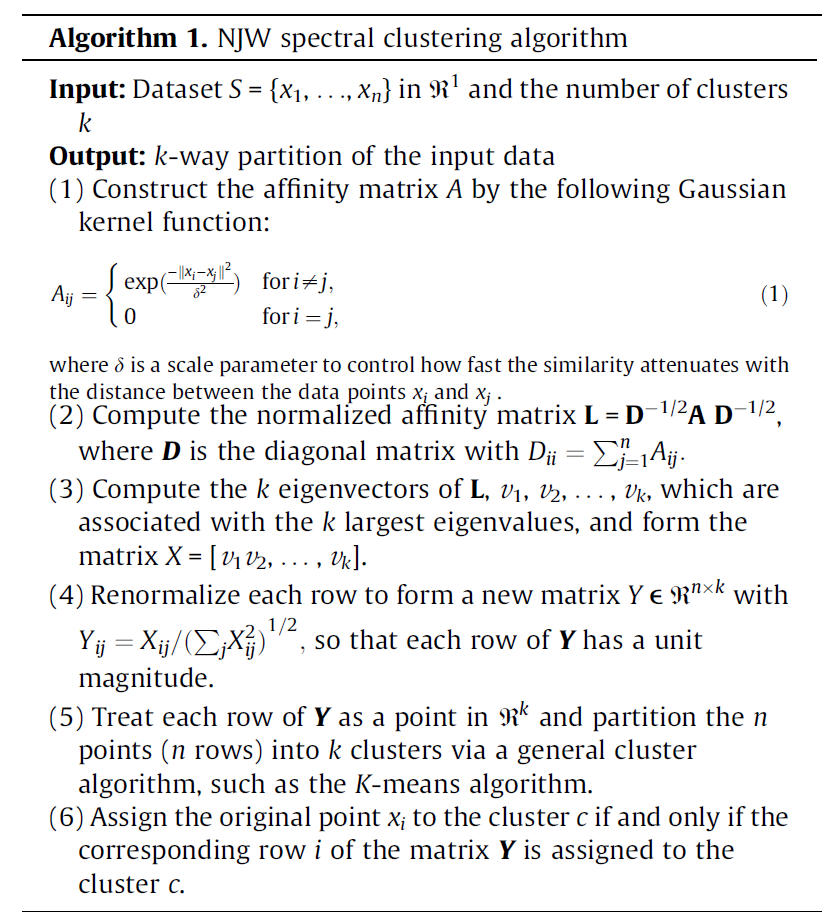
\includegraphics[width = 8cm]{NJW}
\end{figure}


\end{frame}

\begin{frame}
\frametitle{KASP}
  \begin{itemize}
  \item Create a representative set
    \item Spectral cluster representative set 
      \item Assign labels to all original data
  \end{itemize}


%How can we summarise the data to run spectral clustering? \\ \\
%What can we say about the performance of the clustering on the summarised data compared with the clustering using the full data? 


\end{frame}


\begin{frame}
\frametitle{}
\begin{figure}[h]
  \centering
  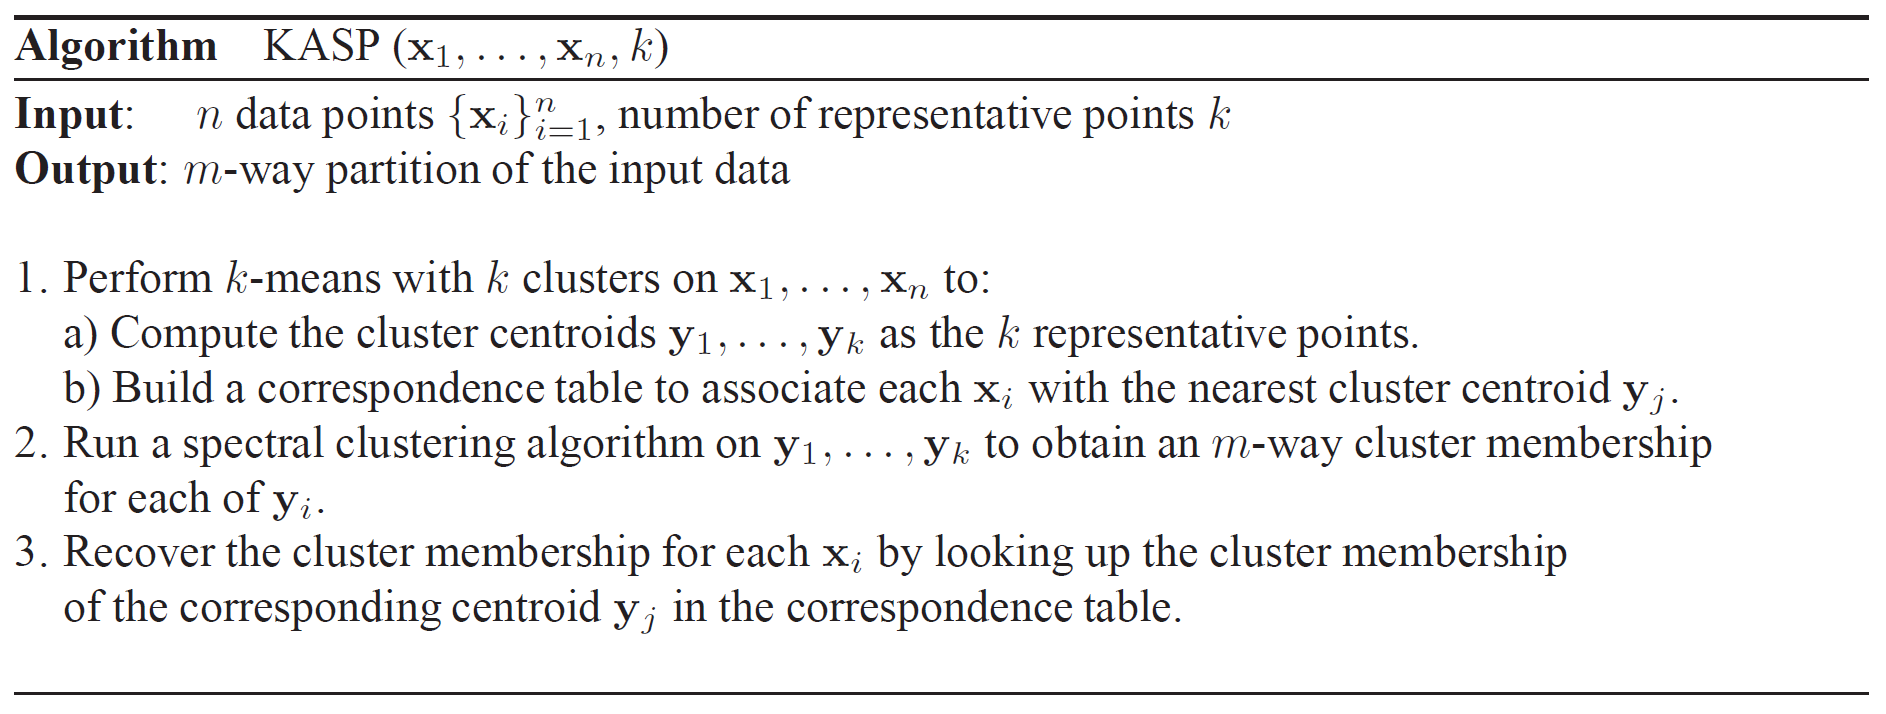
\includegraphics[width = 13cm]{kasp_algo}
\end{figure}
%Discuss Orders
\end{frame}


\begin{frame}
\frametitle{Perturbation Analysis}
Assume $x_1, \ldots, x_n$ i.i.d according to a probability distribution $G$
\begin{equation}
  \label{eq:pert}
  \tilde{x}_i = x_i + \epsilon_i
\end{equation}
$\tilde{x}$ distributed by $\tilde{G}$. 

\begin{itemize}
\item $\epsilon_i$ independent of $x_i$
\item $\epsilon_i$ are i.i.d. according to a symmetric dist (mean zero, bounded support) 
\item Var($\epsilon$) small relative to Var($X$). 
\end{itemize}


\end{frame}

\begin{frame}
\frametitle{Mis-clustering Rate}

\begin{equation}
  \label{eq:misClust}
  \rho = \frac{1}{n} \sum_{i = 1}^{n} \mathbb{I}(I_i \neq \tilde{I}_i)
\end{equation}

%Here $\mathbb{I}$ is the indicator function, $I_i$ represents the cluster allcoated to original datapoint $x_i$ and $\tilde{I_i}$ represents the cluster allocation of perturbed datapoint $\tilde{x}_i$. If $\rho = 1$ then the clustering of the perturbed data is identical to the clustering of the original data. In Section \ref{sec:bounds} we will attempt to justify bounds on the values of the misclustering $rho$ given some understanding of the microclustering process used. 

\end{frame}


\begin{frame}
\frametitle{}

\begin{Theorem}
Under the assumptions(*), the mis-clustering rate $\rho$ of a spectral bi-partitioning algorithm on the perturbed data satisfies
  \begin{equation}
    \label{eq:rho1}
    \rho \leq \| \tilde{v}_2 - v_2 \|^2
  \end{equation}
\end{Theorem}

%Limitations: bi-partition, and only $v_2$

\end{frame}

\begin{frame}
\frametitle{}

\begin{lemma}
Let $g$ denote the eigengap between the second and the third eigenvalues of $L$. Then the following holds:
\begin{equation}
  \label{eq:eigengap}
  \| \tilde{v}_2-v_2 \| \leq \frac{1}{g} \| \tilde{L} - L \| + O(\| \tilde{L} - L \|^2).
\end{equation}
\end{lemma}
%Standard Lemma from Introduction to Matrix Computation (1973 Stewart)
\end{frame}


\begin{frame}
\frametitle{}

\begin{Theorem}
Assume assumptions hold throughout recursive invocation of the Ncut algorithm, $g_0$ is bounded away from zero and Frobenius norm of perturbation of Laplacian matricies along the recursion is bounded by $c\| \tilde{L} - L \|_F^2$ for some constant $c \geq 1$. Then the mis-clustering rate for an $m$-way spectral clustering solution can be bounded by:
  \begin{equation}
    \label{eq:rho1}
    \rho \leq \| \frac{m}{g_0^2} \cdot c \| \tilde{L} - L \|^2_F.
  \end{equation}

\end{Theorem}

\pause

\begin{align*}
r_1 & \leq n \cdot \frac{L_1^2}{g_1^2} \\
r_i & \leq (n - n_{i-1}) \cdot \frac{L_i^2}{g_i^2}, i = 2, \ldots, {m-1}.  
\end{align*}


\end{frame}


\begin{frame}
\frametitle{Linking Laplacian to $\epsilon$}  

\begin{theorem}

  \begin{equation}
    \label{eq:6}
\| \tilde{L} - L \|^2_F \leq_p c_1 \sigma_{\epsilon}^{(2)} + c_2 \sigma_{\epsilon}^{(4)}      
  \end{equation}

\end{theorem}



\end{frame}

\begin{frame}
If we know the probability distribution of the original data, it is possible to characterise the exact amount of distortion. 

f is the density function of G  
\begin{theorem}
  
Let data be distributed with density $f$. 

\begin{equation*}
  \label{eq:kaspBound}
  \rho = c \cdot b_{2,d} \cdot \|f\|_{\frac{d}{d+2}} \cdot k^{-\frac{2}{d}} + O(k^{-\frac{4}{d}})
\end{equation*}

where $c$ is constant determined by number of clusters, variance of original data, bandwidth of Gaussian kernel and the minimum eigengap of all affinity matrices used in Ncut. 

\end{theorem}

\end{frame}

\begin{frame}
\frametitle{#FAIL}
  \begin{figure}[h]
    \centering
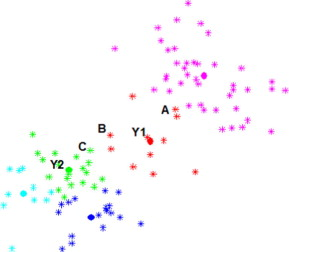
\includegraphics[width = 5cm]{fail}  
  \end{figure}
\end{frame}


\begin{frame}
  \begin{figure}[h]
    \centering
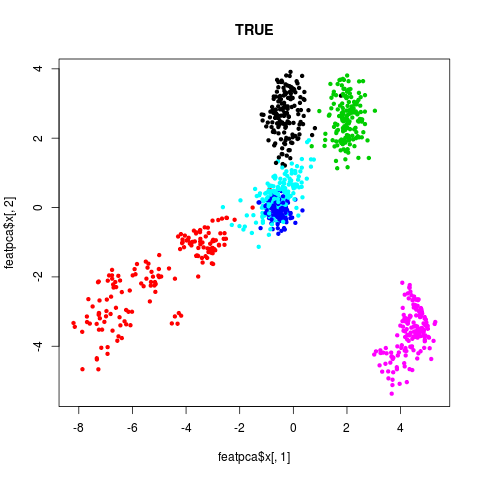
\includegraphics[width = 5cm]{303_true_data}  
  \end{figure}
\end{frame}

\begin{frame}
  \begin{figure}[h]
    \centering
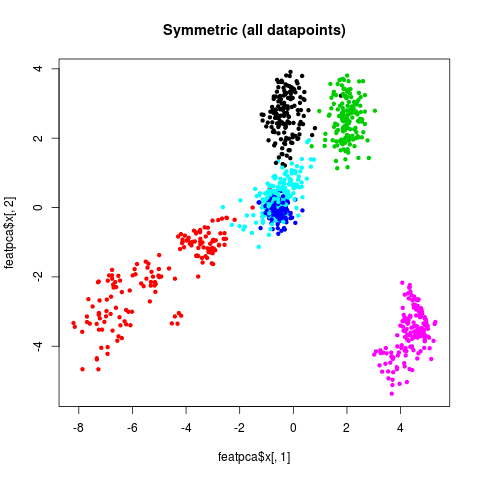
\includegraphics[width = 5cm]{303_s_data}  
  \end{figure}
\end{frame}



%\begin{frame}
%  \includemovie{10cm}{10cm}{303_update_micro.gif}
%\end{frame}


\end{document}